% SUPERSEDED DRAFT (#144): the canonical SoftwareX manuscript is UBC-FRESH/fhops-manuscript.
% This in-repo copy is kept for reference only and is not maintained; do not quote it.
% Numbers come from docs/softwarex/assets (see docs/softwarex/manuscript/README.md).
% FHOPS manuscript (SoftwareX submission wrapper)
\documentclass[preprint,review,12pt]{elsarticle}

\usepackage{hyperref}
\usepackage{amsmath}
\usepackage{amssymb}
\usepackage{textcomp}
\usepackage{lineno}
\usepackage{tikz}
\usetikzlibrary{positioning,arrows.meta}
\usepackage{booktabs}
\usepackage{longtable}
\usepackage{array}
\usepackage{calc}
\modulolinenumbers[5]

\providecommand{\tightlist}{%
  \setlength{\itemsep}{0pt}\setlength{\parskip}{0pt}}

\journal{SoftwareX}

% Shared metadata macros will live here later

\begin{document}

\begin{frontmatter}

\title{FHOPS: a reproducible optimisation and benchmarking stack for forest harvest operations}

\author[ubc]{Gregory Paradis\corref{cor1}}
\cortext[cor1]{Corresponding author: gregory.paradis@ubc.ca}
\address[ubc]{Faculty of Forestry, University of British Columbia, Canada}

% SUPERSEDED DRAFT (#144): the canonical SoftwareX manuscript is UBC-FRESH/fhops-manuscript.
% This in-repo copy is kept for reference only and is not maintained; do not quote it.
% Numbers come from docs/softwarex/assets (see docs/softwarex/manuscript/README.md).
% Highlights placeholder
\section*{Highlights}
\begin{itemize}
  \item FHOPS delivers a full forest-harvest operations workflow (scenario contract, solver stack, telemetry) through a single CLI/API toolkit, providing the same reproducibility signals showcased by recent open-source exemplars.
  \item The same CLI that powers FHOPS deployments also regenerates every dataset, benchmark, tuning study, playback analysis, costing demo, and scaling sweep, logging commit IDs, runtimes, and SHA-256 fingerprints for auditability.
  \item The manuscript scopes its contribution to the open-source platform and documents how forthcoming British Columbia validation studies will reuse the tooling without duplicating context-specific results here.
\end{itemize}


% SUPERSEDED DRAFT (#144): the canonical SoftwareX manuscript is UBC-FRESH/fhops-manuscript.
% This in-repo copy is kept for reference only and is not maintained; do not quote it.
% Numbers come from docs/softwarex/assets (see docs/softwarex/manuscript/README.md).
\begin{abstract}
Forest harvest operations planning still depends on bespoke optimisers, spreadsheet workflows, and undocumented heuristics, even though multiple surveys—including the 2025 systematic review by Jaffray et~al.—have called for reusable tooling. FHOPS answers that gap by packaging the data contract, solver stack (Pyomo MIP plus SA/ILS/Tabu heuristics with Optuna-style tuning), and telemetry/evaluation services that we already run in production. Users can ingest the curated British Columbia ground-based ladder (tiny7→small21→med42) or generate synthetic tiers, run benchmark or playback suites from a single command, and export the resulting tables/figures directly into both this manuscript and the FHOPS Sphinx documentation. Reproducibility is enforced by the same scripted FHOPS pipeline that generates datasets, benchmarks, tuning studies, playback analyses, costing demonstrations, and scaling sweeps while logging commit IDs, runtimes, and SHA-256 fingerprints of the regenerated artifacts. The manuscript therefore scopes its contribution to the open-source platform while outlining how upcoming validation studies (rolling-horizon med42/large84 runs plus skyline/helicopter deployments) will reuse the tooling without duplicating context-specific results here. FHOPS complements existing DSS initiatives (PRISM, lidar-enabled productivity models) by delivering an operations-layer workflow that can be audited, extended, and reused by practitioners and researchers alike.
\end{abstract}


\begin{keyword}
forest operations \sep optimisation \sep reproducibility \sep heuristics \sep Pyomo \sep telemetry
\end{keyword}

% Code metadata table (journal requirement)
% Shared with the canonical manuscript (UBC-FRESH/fhops-manuscript); keep every entry factual:
% platforms = .github/workflows/*.yml, dependencies/floors = pyproject.toml [project].
\begin{table}[ht]
  \centering
  \caption{Code metadata (reproducibility requirement)}
  \label{tab:code-metadata}
  \begin{tabular}{p{0.35\linewidth}p{0.55\linewidth}}
    \hline
    Current code version & FHOPS v1.0.1 (SoftwareX revision release) \\
    Permanent link to code/repository & \url{https://github.com/UBC-FRESH/fhops/tree/v1.0.1} \\
    Legal Code License & MIT License (OSI approved) \\
    Computing platforms/requirements & Python $\geq$ 3.11 on any platform with the PyPI dependencies; developed and tested on GNU/Linux (Ubuntu 24.04 LTS); CI on GitHub Actions \texttt{ubuntu-latest} only \\
    Installation requirements & \texttt{pip install fhops==1.0.1} (PyPI) installs the dependencies listed in Table~\ref{tab:current-code-version}; HiGHS ships with the \texttt{highspy} wheels. Development install: \texttt{pip install -e ".[dev]"}. \\
    Documentation link & \url{https://fhops.readthedocs.io/en/latest/} \\
    Reproducibility log & \texttt{docs/softwarex/assets/benchmark\_runs.log} records every \texttt{make manuscript-benchmarks} run (commit, runtime, SHA-256 assets hash over the committed asset files); artefacts live under \texttt{docs/softwarex/assets/**}. \\
    Support contact & gregory.paradis@ubc.ca (Faculty of Forestry, UBC) \\
    \hline
  \end{tabular}
\end{table}

% Current code version table (journal requirement)
% Shared with the canonical manuscript (UBC-FRESH/fhops-manuscript); keep every entry factual:
% platforms = .github/workflows/*.yml, dependencies/floors = pyproject.toml [project].
\begin{table}[ht]
  \centering
  \caption{Current code version details}
  \label{tab:current-code-version}
  \begin{tabular}{p{0.35\linewidth}p{0.55\linewidth}}
    \hline
    Software version & FHOPS v1.0.1 (SoftwareX revision release) \\
    Permanent link to executables/code & \url{https://github.com/UBC-FRESH/fhops/releases/tag/v1.0.1} (source archive + wheel) \\
    Operating systems & Pure-Python package (platform-independent wheel); developed and tested on GNU/Linux (Ubuntu 24.04 LTS); CI runs on GitHub Actions \texttt{ubuntu-latest} only (macOS and Windows are not tested) \\
    Dependencies & Python $\geq$ 3.11; typer $\geq$ 0.15.4, rich $\geq$ 13.7.0, pydantic $\geq$ 2.6.0, pandas $\geq$ 2.2.0, numpy $\geq$ 1.26.0, Pyomo $\geq$ 6.9.2, highspy $\geq$ 1.8.1 (HiGHS, PyPI wheels), pyarrow $\geq$ 15.0.0, PyYAML $\geq$ 6.0.1, Optuna $\geq$ 3.5.0; optional geopandas $\geq$ 0.14.0 (\texttt{[geo]}) and gurobipy $\geq$ 11.0.0 (\texttt{[gurobi]}) \\
    Installation method & \texttt{pip install fhops==1.0.1} (PyPI); development install \texttt{pip install -e ".[dev]"} \\
    Build system & Hatch / hatchling (PEP~517 backend defined in \texttt{pyproject.toml}) \\
    Continuous integration & GitHub Actions on \texttt{ubuntu-latest} with Python 3.11 (lint, type check, tests, docs): \url{https://github.com/UBC-FRESH/fhops/actions} \\
    Reproducibility evidence & \texttt{make manuscript-benchmarks} regenerates all assets and logs the commit, runtime and an assets hash (recipe documented in \texttt{docs/softwarex/manuscript/README.md}) to \texttt{docs/softwarex/assets/benchmark\_runs.log}; \texttt{make verify-assets-hash} checks it \\
    \hline
  \end{tabular}
\end{table}


\end{frontmatter}

\linenumbers

% SUPERSEDED DRAFT (#144): the canonical SoftwareX manuscript is UBC-FRESH/fhops-manuscript.
% This in-repo copy is kept for reference only and is not maintained; do not quote it.
% Numbers come from docs/softwarex/assets (see docs/softwarex/manuscript/README.md).
% Section 1: Motivation and significance
\section{Motivation and significance}

Modern forest harvesting optimisation problems mirror the increasing complexity highlighted in decades of operations-research and forest-planning literature:\ numerous studies lament that most tools remain bespoke prototypes, tied to a single case study, or hidden behind commercial black boxes \cite{henkelman1978gpssv,weintraub1996new,heinimann2007forest,buongiorno2003decision,kangas2008decision}. Recent reviews reiterate this: despite progress in vehicle-routing decision support \cite{audy2023planning}, PRISM-like DSS stacks \cite{nguyen2022prism}, and ecosystem-view planning frameworks \cite{labarre2025improve}, practitioners still stitch together spreadsheets, GIS workflows, and siloed simulators \cite{ulvdal2022uncertainty,nelson2003forestmodels}. Every new scenario (e.g., introducing skyline systems, injecting salvage corridors, calibrating productivity models) triggers a bespoke analysis loop.

Jaffray et~al.’s systematic review of operational-planning models catalogues the practical consequences of that fragmentation (Section~4, Tables~3–4) \cite{jaffray2025systematic}: (i) fewer than 10\,\% of the 140+ studies surveyed ship reusable code or data; (ii) solver designs are highly site-specific, making it difficult to compare heuristics across coastal skyline, tethered/steep-slope, helicopter, and ground-based systems; and (iii) reproducibility is rarely demonstrated, with evaluation scripts or telemetry traces almost never released. The review concludes that BC’s diverse operational contexts—steep coastal skylines, small- and large-tenure ground systems, and emerging salvage programs—require a reusable workflow that can ingest heterogeneous scenario contracts, apply multiple solver families, and publish the resulting telemetry so that follow-on validation studies can build from a stable foundation instead of starting from scratch.

Recent open-source exemplars such as PyLESA, pycity\_scheduling, cashocs, PyDDRBG, GROMACS, and libxc illustrate the standard we need to meet: they lead with metadata tables, document automation hooks, ship benchmark manifests, and describe governance processes so readers can trust the project’s longevity \cite{Lyden2021PyLESA,Schwarz2021pycity,Blauth2023cashocs,Ahrari2022PyDDRBG,Abraham2015GROMACS,Lehtola2018libxc}. Those papers emphasise a repeatable workflow—architecture diagrams, scripted experiments, artefact hashes—and couple it with adoption evidence (downstream users, release cadence). FHOPS mirrors that playbook: the manuscript reuses the same CLI automation, dataset catalogue, and telemetry logs that power the public documentation set, ensuring this is not a one-off branch but the canonical release pipeline.

FHOPS targets these persistent gaps by packaging the optimisation heuristics, MIP constructs, scenario contract, and evaluation telemetry we already operate in production into a single, research-friendly stack. Like PyLESA, we state explicit gaps up front—multi-problem workflows, telemetry-backed reproducibility, solver governance, shared datasets—and show how FHOPS compresses the “scoping → benchmarking → deployment” loop for harvesting teams. Our aim is complementary to open-source initiatives in forest planning (e.g., PRISM, lidar-enabled harvest-system selection, productivity syntheses) \cite{nguyen2022prism,becker2018lidar,lahrsen2022productivity}: FHOPS focuses on the operations layer, wrapping tactical/operational problem classes into a reusable pipeline and exposing them as Typer CLI + Python APIs.

The codebase has only just been published outside the UBC FRESH lab: \texttt{v1.0.0} is the first stable public tag and the benchmark suite presented here was generated within weeks of submission. Prior internal projects informed the architecture, but there is not yet a broad downstream user base or long release history to cite. We document FHOPS now precisely because the reproducibility scaffolding is in place and the forthcoming BC deployments require a stable, citable artefact; the manuscript therefore emphasises transparent automation instead of retrospective adoption statistics.

Tables~\ref{tab:code-metadata} and \ref{tab:current-code-version} capture the reproducibility metadata expected by the journal: the specific FHOPS release (\texttt{v1.0.1}, a maintenance release on the stable 1.0 line), licence, platform support, installation method, and the benchmark log path (\texttt{docs/softwarex/assets/benchmark\_runs.log}) that records every regeneration run. By presenting those tables up front we signal the provenance of every asset cited later in the manuscript and make it explicit that other researchers can reproduce the exact snapshot referenced here.

Throughout the manuscript we reference concrete CLI entry points and asset directories so readers can map each narrative block back to a command and output path. For example, Section~\ref{sec:software-description} cites the dataset validator (`fhops validate examples/tiny7/scenario.yaml`), the benchmark harness (`fhops bench suite --scenario ... --out-dir docs/softwarex/assets/data/benchmarks/<slug>`), and the playback tooling (`fhops eval-playback ... --day-out docs/softwarex/assets/data/playback/<slug>/<solver>/<mode>/day.csv`). Section~\ref{sec:illustrative-example} then reuses those exact paths when presenting Tables~\ref{tab:benchmarks}--\ref{tab:tuning} and Figures~\ref{fig:playback}--\ref{fig:scaling}, ensuring every number in the manuscript can be traced back to a CSV/JSON/PNG under \texttt{docs/softwarex/assets/}.

The manuscript therefore makes three contributions:
1. **Architecture + data contract** – We formalise the FHOPS architecture (scenario ingestion, optimisation services, telemetry) so planners can reason about model scope and reproduce results outside our internal environment. Shared includes capture the metadata, harvest-system registry, and scenario schemas so the manuscript, Sphinx docs, and CLI help stay in lockstep—mirroring the clarity PyLESA and pycity\_scheduling offer for energy-system modelling \cite{Lyden2021PyLESA,Schwarz2021pycity}.
2. **Benchmark + reproducibility tooling** – We publish a benchmark matrix (scheduling, routing, resource allocation) with scripts that regenerate KPI tables/plots via one command, following the best practices PyDDRBG and cashocs established \cite{Ahrari2022PyDDRBG,Blauth2023cashocs}. Tables~\ref{tab:benchmarks}--\ref{tab:tuning} and Figures~\ref{fig:playback}--\ref{fig:scaling} are auto-generated from the same CLI pipeline readers run locally.
3. **Governance + adoption evidence** – We document the governance model (release cadence, contributor process, validation suite) so stakeholders know how FHOPS will be maintained as external case studies come online, mirroring the transparency seen in libxc/MOOSE/GROMACS \cite{Lehtola2018libxc,Permann2020MOOSE,Abraham2015GROMACS}. The metadata tables explicitly record licence, support channels, and linkage to the stable release tag (\texttt{v1.0.1}) archived with this manuscript, giving future users a stable anchor even at this early stage.

By design we keep this contribution focused on the reusable platform. The detailed deployment of FHOPS on multiple British Columbia case studies (e.g., skyline corridors, salvage operations, small tenure planning) is being prepared as separate validation studies, ensuring those analyses retain their own novelty while leveraging the shared tooling documented here. That separation lets FHOPS cite the systematic review’s gaps while reserving the upcoming BC-specific analyses for future domain publications.

Section~\ref{sec:software-description} decomposes the software into ingest, optimisation, and evaluation layers and shows how they interact with the open data catalogue. Section~\ref{sec:illustrative-example} walks through a benchmark suite spanning three optimisation classes and the telemetry/CI hooks that keep it reproducible. Section~\ref{sec:impact} quantifies adoption plus governance processes inspired by libxc/MOOSE, and we close with the roadmap and submission logistics to keep FHOPS aligned with the reproducibility signals highlighted by prior exemplar papers \cite{Blauth2023cashocs}.

% SUPERSEDED DRAFT (#144): the canonical SoftwareX manuscript is UBC-FRESH/fhops-manuscript.
% This in-repo copy is kept for reference only and is not maintained; do not quote it.
% Numbers come from docs/softwarex/assets (see docs/softwarex/manuscript/README.md).
% Section 2: Software description
\section{Software description}
\label{sec:software-description}

\textbf{Overview.} FHOPS ships as a Python package backed by Typer-based CLI tooling and a data contract that keeps datasets, solver inputs, and telemetry consistent. The system breaks down into three layers, each callable via CLI (\texttt{fhops.cli.*}) or Python APIs, so users can script the workflow end-to-end or embed modules inside downstream DSS projects:

\begin{enumerate}
  \item \textbf{Data ingest \& scenario contract} – schema + loaders that convert CSV/YAML datasets into typed \texttt{Scenario} objects.
  \item \textbf{Optimisation services} – heuristics (SA/ILS/Tabu), MIP builder, and evaluation harness.
  \item \textbf{Telemetry \& assets} – reproducible logging, benchmark scripts, figure/table generation.
\end{enumerate}

Each layer is consumable via API or CLI, mirroring the dual entry points emphasized in pycity\_scheduling, TSFEL, and contemporary forest-planning DSS (e.g., PRISM, multi-attribute spatial tools) \cite{nguyen2022prism,kuhmaier2010dss}. Internally the packages mirror this structure: scenario models sit under \texttt{fhops.scenario.contract} / \texttt{fhops.scenario.synthetic}, optimisation logic under \texttt{fhops.optimization} (heuristics and Pyomo builder), and evaluation/telemetry helpers under \texttt{fhops.evaluation} and \texttt{fhops.telemetry}. The CLI wrappers (\texttt{fhops.cli.*}) simply call these modules, so referencing a function in the manuscript maps 1:1 to a Python module path that downstream developers can import.

Figure~\ref{fig:fhops-prisma-overview} summarises the automation pipeline that underpins this layered design. The PRISMA-style diagram follows the data from scenario contracts and curated datasets through FHOPS’ ingest, solver, tuning, and telemetry components, then out to benchmark/playback artefacts that readers can reproduce with the same CLI sequence. It visually reinforces that FHOPS treats reproducibility as part of the core platform rather than an add-on.

\begin{figure}[t]
  \centering
  \resizebox{\linewidth}{!}{%
  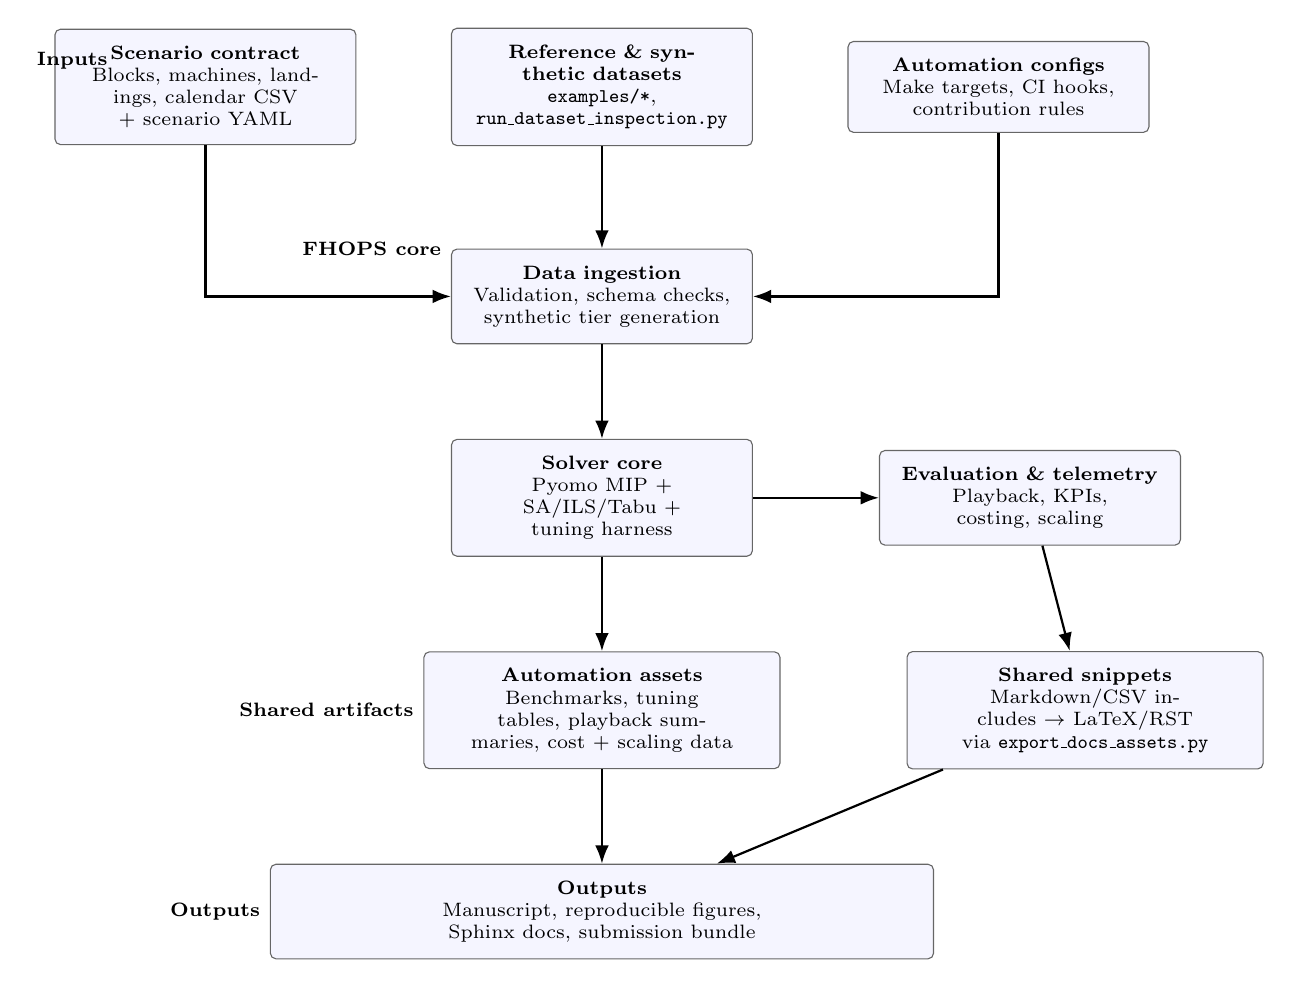
\begin{tikzpicture}[
    font=\scriptsize,
    node distance=1.5cm,
    block/.style={rectangle, rounded corners=2pt, draw=black!60, fill=blue!4, align=center, text width=3.4cm, inner sep=6pt},
    wideblock/.style={block, text width=4.1cm},
    arrow/.style={-Latex, thick},
    labelnode/.style={font=\scriptsize\bfseries, anchor=west}
  ]
    % Inputs
    \node[block] (in1) {\textbf{Scenario contract}\\Blocks, machines, landings, calendar CSV + scenario YAML};
    \node[block, right=1.2cm of in1] (in2) {\textbf{Reference \& synthetic datasets}\\\texttt{examples/*}, \texttt{run\_dataset\_inspection.py}};
    \node[block, right=1.2cm of in2] (in3) {\textbf{Automation configs}\\Make targets, CI hooks, contribution rules};
    \node[labelnode, above left=0.1cm and -0.8cm of in1.west] {Inputs};

    % Core
    \node[block, below=1.3cm of in2] (core1) {\textbf{Data ingestion}\\Validation, schema checks, synthetic tier generation};
    \node[block, below=1.2cm of core1] (core2) {\textbf{Solver core}\\Pyomo MIP + SA/ILS/Tabu + tuning harness};
    \node[block, right=1.6cm of core2] (core3) {\textbf{Evaluation \& telemetry}\\Playback, KPIs, costing, scaling};
    \node[labelnode, left=0cm of core1.west, align=left, yshift=0.6cm] {FHOPS core};

    % Shared outputs
    \node[wideblock, below=1.2cm of core2] (int1) {\textbf{Automation assets}\\Benchmarks, tuning tables, playback summaries, cost + scaling data};
    \node[wideblock, right=1.6cm of int1] (int2) {\textbf{Shared snippets}\\Markdown/CSV includes $\rightarrow$ LaTeX/RST via \texttt{export\_docs\_assets.py}};
    \node[labelnode, left=0cm of int1.west] {Shared artifacts};

    % Final outputs
    \node[wideblock, below=1.2cm of int1, text width=8cm] (out1) {\textbf{Outputs}\\Manuscript, reproducible figures, Sphinx docs, submission bundle};
    \node[labelnode, left=0cm of out1.west] {Outputs};

    % Connections
    \draw[arrow] (in1) |- (core1);
    \draw[arrow] (in2) -- (core1);
    \draw[arrow] (in3) |- (core1);
    \draw[arrow] (core1) -- (core2);
    \draw[arrow] (core2) -- (core3);
    \draw[arrow] (core2) -- (int1);
    \draw[arrow] (core3) -- (int2);
    \draw[arrow] (int1) -- (out1);
    \draw[arrow] (int2) -- (out1);
  \end{tikzpicture}%
  }
  \caption{FHOPS automation pipeline. Inputs (scenario contract + curated datasets) feed the FHOPS core (validation, solver stack, evaluation tooling). Asset scripts emit shared tables/figures consumed by the manuscript, submission package, and Sphinx docs.}
  \label{fig:fhops-prisma-overview}
\end{figure}


\subsection{Data ingest and scenario contract}
\textbf{Components.}
\begin{itemize}
  \item Reference dataset ladder – FHOPS ships three ground-based bundles (`examples/tiny7`, `examples/small21`, `examples/med42`) that share the same harvest-system archetype but scale horizon length, machine counts, and mobilisation footprints. Large84 introduces two concurrent systems and remains a stress-case reserved for future rolling-horizon demonstrations, so it stays out of the reproducibility tables until we can solve it deterministically.
  \item \texttt{fhops.scenario.contract} – Pydantic-based models encode blocks, machines, corridors, mobilisation jobs, and shift calendars. Each schema element enforces unit-checked payloads, terrain classes, prescription types, and per-shift KPI fields, following the BC-focused constraints described by \cite{lahrsen2022productivity} and \cite{becker2018lidar}.
  \item Dataset loaders (\texttt{fhops.cli.dataset}) – convert CSV/YAML bundles (e.g., TN-147 skyline corridors, TR-122 Roberts Creek blocks, med42 reference dataset) into typed \texttt{Scenario} objects. The loader emits validation reports (e.g., `fhops validate examples/tiny7/scenario.yaml`) and canonicalises IDs so solvers and playback routines can consume them deterministically.
  \item Synthetic generator (\texttt{fhops.scenario.synthetic}) – produces stratified scenarios (e.g., \texttt{fhops synth generate out/synthetic\_small --tier small --seed 101 --overwrite}) with configurable harvest-system mixes, blackout biases, and sample counts. These synthetic tiers underpin the scaling experiments and provide shareable exemplars when real datasets remain private.
  \item Hooks for forthcoming BC validation datasets (ground-based, skyline, tethered, and salvage systems). The interface already supports alternative block layouts and mobilisation constraints so companion studies can drop their data in without modifying FHOPS core.
\end{itemize}

\textbf{Dependencies.} Pydantic for schema enforcement, pandas/numpy for CSV IO, PyYAML for scenario files, pyarrow for Parquet.

\textbf{Outputs.} Validated \texttt{Scenario} objects plus manifest metadata: harvest-system inventories, road/mobilisation task tables, calendar definitions, and JSON summaries consumed by the benchmark/playback tools. Each ingest run writes a summary JSON to the user-specified output directory (e.g., `docs/softwarex/assets/data/datasets/`) so the dataset composition cited in Section~\ref{sec:illustrative-example} can be inspected or versioned.

\subsection{Optimisation services}
\textbf{Components.}
\begin{itemize}
  \item Heuristics under \texttt{fhops.optimization.heuristics} – Simulated Annealing (SA), Iterated Local Search (ILS), and Tabu search implemented with pluggable operator weights and temperature schedules. Each solver exposes Typer entry points (\texttt{fhops solve-heur}, \texttt{fhops solve-ils}, \texttt{fhops solve-tabu}, and \texttt{fhops bench suite --include-ils --include-tabu}, which always runs SA) and shares productivity lookup tables parameterised by empirical studies \cite{lahrsen2022productivity,becker2018lidar}. Parallel multi-start runs are production-ready, while within-run batched neighbour evaluation exists but remains GIL-bound today; incremental “move diff” scoring keeps proposals cheap while we experiment with faster executors.
  \item Tuning harness – FHOPS ships a companion tuning runner that executes random, grid, Bayesian, ILS, and Tabu parameter sweeps across multiple scenarios. It emits leaderboard summaries and telemetry logs so users can compare heuristics with the same instrumentation used for the manuscript benchmarks. The manuscript assets use fixed tuning budgets (120 SA iterations per configuration, 8 Bayesian trials, ILS 160 / Tabu 900 iterations) whether or not the asset pipeline runs with \texttt{FHOPS\_ASSETS\_FAST=1}, which only shortens the benchmark budgets.
  \item MIP builder (\texttt{fhops.optimization.mip}) – single-level, shift-based Pyomo formulation solved with HiGHS, borrowing structural ideas (capacity coupling, mobilisation sequencing) from classical bilevel/multi-period harvest models \cite{paradis2018bilevel,nelson2003forestmodels}. Provides an exact baseline when heuristics are insufficient. Warm-start plumbing is fully wired (CLI \texttt{--incumbent} + bundle dumps) even though practical wins on med42 are still limited; the infrastructure is ready for forthcoming rolling-horizon experiments and solver tuning.
  \item Playback + KPI generation (\texttt{fhops.evaluation.playback} / \texttt{fhops.evaluation.metrics}) – replays solver output deterministically or with stochastic shocks (downtime, weather, landing congestion) to compute shift/day KPIs, utilisation, and cost metrics.
\end{itemize}

\textbf{Dependencies.} numpy, Pyomo with HiGHS via highspy (exact solver), Typer/Click/Rich for CLI ergonomics, Optuna for Bayesian tuning, pandas for CSV summaries.

\textbf{Outputs.} Each solver/tuning run produces a summary (objective, runtime, assignments), per-iteration telemetry, and optional playback/cost reports through the standard FHOPS CLI. Users control the destination via \texttt{--out-dir} and related flags—e.g., `fhops bench suite --scenario examples/med42/scenario.yaml --out-dir docs/softwarex/assets/data/benchmarks/med42 --telemetry-log ...`—so assets can be archived, compared, or re-ingested by downstream tools. These same artifacts underpin the illustrative example in Section~\ref{sec:illustrative-example}.

\subsubsection*{Mixed-integer programming baseline}
% AUTO-GENERATED from fhops_operational_formulation.md -- do not edit directly.
FHOPS' deterministic operational solver is formulated on a day-shift
grid and maximizes weighted delivered production while penalizing
leftovers, landing over-capacity slack, and machine movement costs. The
equations below mirror the implemented Pyomo model in
\texttt{fhops.model.milp.operational.build\_operational\_model} and the
bundle normalization in
\texttt{fhops.model.milp.data.build\_operational\_bundle}.

\textbf{Problem statement.} Given harvest blocks, machine roles, shift
calendars, block windows, landing capacities, and harvest-system role
prerequisites, choose machine-block assignments and per-shift production
quantities to maximize weighted production subject to feasibility and
sequencing constraints.

\textbf{Sets and indices.}

\begin{itemize}
\tightlist
\item
  \(m \in \mathcal{M}\): machines.
\item
  \(b \in \mathcal{B}\): blocks.
\item
  \(s=(d,\sigma) \in \mathcal{S}\): shift slots indexed by day
  \(d \in \mathcal{D}\) and shift label \(\sigma\), ordered by day and,
  within a day, by the scenario's shift order;
  \(\operatorname{prev}(s)\) is the preceding slot (the previous shift
  of the same day when there is one) and \(s'\prec s\) means slot \(s'\)
  precedes \(s\).
\item
  \(\mathcal{B}^{\text{seq}} \subseteq \mathcal{B}\): blocks with an
  explicit harvest system (\texttt{harvest\_system\_id}); blocks in
  \(\mathcal{B}\setminus\mathcal{B}^{\text{seq}}\) carry no sequencing
  obligations.
\item
  \(\mathcal{R}_b\): ordered machine roles required by the harvest
  system assigned to block \(b\in\mathcal{B}^{\text{seq}}\)
  (\(\mathcal{R}_b=\emptyset\) otherwise).
\item
  \(\mathcal{L}\): landings.
\item
  \(\mathcal{P}^{\text{inv}} \subseteq \{(r,b): r \in \mathcal{R}_b\}\):
  role-block pairs with upstream prerequisites.
\item
  \(\mathcal{P}^{\text{act}} \subseteq \mathcal{P}^{\text{inv}}\):
  role-block pairs that require positive head-start buffer activation.
\item
  \(\mathcal{P}^{\text{hs}} \subseteq \mathcal{P}^{\text{act}}\): pairs
  with a head start of \(\beta_{r,b}>0\) shifts
  (\texttt{role\_headstart\_shifts}); loader pairs without a head start
  are in \(\mathcal{P}^{\text{act}}\setminus\mathcal{P}^{\text{hs}}\).
\item
  \(\mathcal{P}^{\text{load}} \subseteq \{(r,b): r \in \mathcal{R}_b\}\):
  loader role-block pairs.
\item
  \(s_1 \in \mathcal{S}\): first shift slot of the horizon.
\item
  \(\mathcal{M}^{0} \subseteq \mathcal{M}\): machines with a known
  initial block \(b^{0}_m\) (optional initial state; empty by default).
\item
  \(\mathcal{K}\): locked assignments \(k=(m_k,b_k,d_k,\sigma_k)\),
  where \(\sigma_k\) is a shift label or empty (whole day);
  \(\mathcal{S}_k = \{s=(d_k,\sigma) \in \mathcal{S} : \sigma_k \text{ empty or } \sigma=\sigma_k\}\)
  (empty by default).
\end{itemize}

\textbf{Parameters.}

\begin{itemize}
\tightlist
\item
  \(\bar{p}_{mb}\): production rate for machine \(m\) on block \(b\)
  (units per shift).
\item
  \(W_b\): required total block production volume.
\item
  \(A_{m,s} \in \{0,1\}\): machine availability for shift \(s\).
\item
  \(\mathbf{1}^{\text{window}}_{b,d} \in \{0,1\}\): block window
  indicator (1 if day \(d\) is within block \(b\) window).
\item
  \(\omega^{\text{prod}},\omega^{\text{mob}},\omega^{\text{trans}},\omega^{\text{land}}\):
  objective weights.
\item
  \(\delta_{m,b',b}\): mobilization cost when machine \(m\) transitions
  from block \(b'\) to block \(b\).
\item
  \(C_{\ell}\): daily assignment capacity for landing \(\ell\).
\item
  \(\ell(b)\): landing associated with block \(b\).
\item
  \(\mathcal{U}_{r,b}\): upstream roles that must feed role \(r\) on
  block \(b\).
\item
  \(B_{r,b}\): required staged buffer volume before role \(r\) may
  activate on block \(b\):
  \(B_{r,b}=\beta_{r,b}\sum_{u\in\mathcal{U}_{r,b}}\sum_{m\in\mathcal{M}(u)}\bar{p}_{mb}\)
  for a head start of \(\beta_{r,b}\) shifts
  (\texttt{role\_headstart\_shifts}, 0 by default); loader roles use
  \(\max\{\beta_{r,b}\sum_{u\in\mathcal{U}_{r,b}}\sum_{m\in\mathcal{M}(u)}\bar{p}_{mb},\; \min(q^{\text{batch}}_{r,b}, R_{r,b})\}\)
  (one truckload staged, or the whole remaining block volume when it is
  smaller).
\item
  \(Q_{r,b}\): role production capacity upper bound per shift (used for
  activation linearization).
\item
  \(q^{\text{batch}}_{r,b}\): loader batch size for loader role \(r\) on
  block \(b\).
\item
  \(\mathcal{T}_b \subseteq \mathcal{R}_b\): terminal roles for block
  \(b\) (roles credited in block completion objective terms).
\item
  \(\bar{I}_{u,b} \ge 0\): initial staged volume output by role \(u\) on
  block \(b\) and not yet consumed downstream (optional initial state; 0
  by default).
\item
  \(I^{0}_{r,b} = \min_{u\in\mathcal{U}_{r,b}} \bar{I}_{u,b}\): initial
  input inventory available to downstream role \(r\) on block \(b\) (0
  by default).
\item
  \(R_{r,b} \ge 0\): remaining volume role \(r\) may still output on
  block \(b\): the carried-in value when the optional initial state
  supplies one, otherwise \(W_b\) (every role handles the same wood).
\item
  \(b^{0}_m\): block machine \(m\in\mathcal{M}^{0}\) occupied in its
  last worked slot before the horizon.
\end{itemize}

\textbf{Decision variables.}

\begin{itemize}
\tightlist
\item
  \(x_{m,b,s} \in \{0,1\}\): 1 if machine \(m\) is assigned to block
  \(b\) in shift \(s\).
\item
  \(p_{m,b,s} \ge 0\): production by machine \(m\) on block \(b\) in
  shift \(s\).
\item
  \(z_{r,b,s} \ge 0\): aggregated role-level production for role \(r\)
  on block \(b\) in shift \(s\).
\item
  \(y_{m,b',b,s} \in \{0,1\}\): transition indicator for machine \(m\)
  from previous-shift block \(b'\) to current block \(b\) (defined for
  non-initial shifts).
\item
  \(I^{\text{start}}_{r,b,s} \ge 0\): staged inventory available at
  start of shift \(s\) for role \(r\) on block \(b\).
\item
  \(I_{r,b,s} \ge 0\): staged inventory at end of shift \(s\) for role
  \(r\) on block \(b\).
\item
  \(g_{r,b,s} \in \{0,1\}\): role activation indicator for buffered
  downstream roles.
\item
  \(h_{r,b,s} \in \{0,1\}\), \((r,b)\in\mathcal{P}^{\text{hs}}\): 1 only
  if every upstream role of \(r\) on block \(b\) has output its whole
  remaining volume before slot \(s\) (the buffer can no longer grow and
  is waived).
\item
  \(n_{r,b,s} \in \mathbb{Z}_{\ge 0}\): loader batch count for loader
  role-block pair \((r,b)\).
\item
  \(u_{r,b,s} \ge 0\): loader partial remainder volume.
\item
  \(L_b \ge 0\): leftover unmet block volume slack.
\item
  \(S_{\ell,d} \ge 0\): landing daily surplus slack.
\end{itemize}

\textbf{Objective.}

FHOPS maximizes weighted terminal production and subtracts penalty
terms:

\[
\begin{aligned}
\max\; &\omega^{\text{prod}}\!\sum_{b\in\mathcal{B}}\sum_{r\in\mathcal{T}_b}\sum_{s\in\mathcal{S}} z_{r,b,s}
- \omega^{\text{prod}}\!\sum_{b\in\mathcal{B}} L_b \\
&- \omega^{\text{land}}\!\sum_{\ell\in\mathcal{L}}\sum_{d\in\mathcal{D}} S_{\ell,d} \\
&- \omega^{\text{mob}}\!\sum_{m,b',b,s} \delta_{m,b',b}\, y_{m,b',b,s}
- \omega^{\text{trans}}\!\sum_{m,b',b,s} y_{m,b',b,s} \\
&- \sum_{m\in\mathcal{M}^{0}}\sum_{b\in\mathcal{B}\setminus\{b^{0}_m\}}
\left(\omega^{\text{mob}}\,\delta_{m,b^{0}_m,b} + \omega^{\text{trans}}\right) x_{m,b,s_1}.
\end{aligned}
\]

The last line is the boundary transition from each machine's initial
block into the first slot. It is linear in \(x\) because \(b^{0}_m\) is
data; with no initial state (\(\mathcal{M}^{0}=\emptyset\)) it vanishes
and the objective is the v1.0.0 objective.

For blocks without terminal roles (\(\mathcal{T}_b=\emptyset\), in
particular blocks outside \(\mathcal{B}^{\text{seq}}\)) the production
reward and the block balance use the machine-level sum
\(\sum_{m}\sum_{s} p_{m,b,s}\) in place of
\(\sum_{r\in\mathcal{T}_b}\sum_s z_{r,b,s}\).

\textbf{Constraints.}

Machine assignment feasibility:

\[
\sum_{b\in\mathcal{B}} x_{m,b,s} \le A_{m,s}
\qquad \forall m\in\mathcal{M},\; s\in\mathcal{S}.
\]

Role compatibility (machines can only work roles allowed by the block's
assigned harvest system):

\[
x_{m,b,s}=0 \quad \text{if } b\in\mathcal{B}^{\text{seq}} \text{ and role}(m)\notin\mathcal{R}_b.
\]

Production upper bound per assignment:

\[
p_{m,b,s} \le \bar{p}_{mb}\,x_{m,b,s}
\qquad \forall m,b,s.
\]

Block window enforcement:

\[
x_{m,b,s}=0 \quad \text{if } \mathbf{1}^{\text{window}}_{b,d}=0 \text{ for } s=(d,\sigma).
\]

Role-production aggregation:

\[
z_{r,b,s} = \sum_{m\in\mathcal{M}(r)} p_{m,b,s}
\qquad \forall (r,b), s.
\]

Transition linking (for non-initial shifts only):

\[
y_{m,b',b,s} \le x_{m,b',\operatorname{prev}(s)},
\qquad
y_{m,b',b,s} \le x_{m,b,s},
\] \[
y_{m,b',b,s} \ge x_{m,b',\operatorname{prev}(s)} + x_{m,b,s} - 1.
\]

Role inventory start and balance for prerequisite-driven downstream
roles:

\[
I^{\text{start}}_{r,b,s}=
\begin{cases}
I^{0}_{r,b}, & s = s_1\\
I_{r,b,\operatorname{prev}(s)}, & \text{otherwise}
\end{cases}
\qquad \forall (r,b)\in\mathcal{P}^{\text{inv}}, s,
\]

\[
I_{r,b,s}=I^{\text{start}}_{r,b,s}+\sum_{u\in\mathcal{U}_{r,b}} z_{u,b,s}-z_{r,b,s}
\qquad \forall (r,b)\in\mathcal{P}^{\text{inv}}, s,
\]

\[
z_{r,b,s} \le I^{\text{start}}_{r,b,s}
\qquad \forall (r,b)\in\mathcal{P}^{\text{inv}}, s.
\]

Head-start activation for buffered downstream roles:

\[
z_{r,b,s} \le Q_{r,b}\,g_{r,b,s}
\qquad \forall (r,b)\in\mathcal{P}^{\text{act}}, s,
\]

\[
I_{r,b,\operatorname{prev}(s)} \ge B_{r,b}\,g_{r,b,s}
\qquad \forall (r,b)\in\mathcal{P}^{\text{act}}\setminus\mathcal{P}^{\text{hs}}, s,
\qquad
I_{r,b,\operatorname{prev}(s)} \ge B_{r,b}\,\left(g_{r,b,s}-h_{r,b,s}\right)
\qquad \forall (r,b)\in\mathcal{P}^{\text{hs}}, s,
\]

with \(I_{r,b,\operatorname{prev}(s_1)} := I^{0}_{r,b}\), and

\[
\sum_{s'\prec s} z_{u,b,s'} \ge R_{u,b}\,h_{r,b,s}
\qquad \forall (r,b)\in\mathcal{P}^{\text{hs}},\; u\in\mathcal{U}_{r,b},\; s,
\]

\[
\sum_{m\in\mathcal{M}(r)} x_{m,b,s} \le |\mathcal{M}(r)|\, g_{r,b,s},
\qquad
g_{r,b,s} \le \sum_{m\in\mathcal{M}(r)} x_{m,b,s}
\qquad \forall (r,b)\in\mathcal{P}^{\text{act}}, s.
\]

Loader batching:

\[
z_{r,b,s}=q^{\text{batch}}_{r,b}\,n_{r,b,s}+u_{r,b,s}
\qquad \forall (r,b)\in\mathcal{P}^{\text{load}}, s,
\]

\[
0 \le u_{r,b,s} \le q^{\text{batch}}_{r,b}
\qquad \forall (r,b)\in\mathcal{P}^{\text{load}}, s.
\]

Block completion balance with leftover slack:

\[
\sum_{r\in\mathcal{T}_b}\sum_{s\in\mathcal{S}} z_{r,b,s} + L_b = W_b
\qquad \forall b\in\mathcal{B}.
\]

Remaining role output (no role can handle more wood than the block still
holds):

\[
\sum_{s\in\mathcal{S}} z_{r,b,s} \le R_{r,b}
\qquad \forall b\in\mathcal{B}^{\text{seq}},\; r\in\mathcal{R}_b.
\]

Locked assignments (a lock without a shift label pins every available
shift of its day; a lock with a shift label pins only that slot):

\[
x_{m_k,b,s} = A_{m_k,s}\,\mathbf{1}[b=b_k]
\qquad \forall k\in\mathcal{K},\; s\in\mathcal{S}_k,\; b\in\mathcal{B}.
\]

Landing daily assignment capacity with surplus slack:

\[
\sum_{b:\,\ell(b)=\ell}\sum_{m\in\mathcal{M}}\sum_{\sigma:(d,\sigma)\in\mathcal{S}} x_{m,b,(d,\sigma)}
\le C_{\ell} + S_{\ell,d}
\qquad \forall \ell\in\mathcal{L},\; d\in\mathcal{D}.
\]

Domain restrictions:

\[
x, y, g, h \in \{0,1\},\quad n \in \mathbb{Z}_{\ge 0},\quad p,z,I^{\text{start}},I,u,L,S \ge 0.
\]

\textbf{Initial state defaults.} Without
\texttt{Scenario.initial\_state} and
\texttt{Scenario.locked\_assignments} (\(\bar{I}\equiv 0\), hence
\(I^{0}\equiv 0\); \(R_{r,b}\equiv W_b\);
\(\mathcal{M}^{0}=\mathcal{K}=\emptyset\)) the initial-state and lock
terms vanish.

\textbf{Changes from FHOPS v1.0.0 (1.0.1).} Three corrections make every
MILP plan physically feasible and replayable by the playback sequencing
tracker without violations: (i) the remaining-output cap now applies to
every role with \(R_{r,b}=W_b\) by default (v1.0.0 let upstream roles
output more volume than the block holds and used that volume to meet
head-start and loader thresholds); (ii) the head-start constraint of
roles with a head start is waived through \(h_{r,b,s}\) once every
upstream role has output its whole remaining volume, and the loader
threshold is \(\min(q^{\text{batch}}_{r,b}, R_{r,b})\), so blocks
smaller than a buffer or a truckload can still be finished without the
excess volume; (iii) blocks without a harvest system
(\(\mathcal{B}\setminus\mathcal{B}^{\text{seq}}\)) have no role
obligations, as documented in the data contract (v1.0.0 applied the
registry's default system to them). Playback, the heuristics, and the
rolling-horizon carry-forward apply the same rules: staged output is
available from the next shift slot, buffers are staged volume at the
start of the slot, and production is capped by \(R_{r,b}\).

\textbf{Implementation mapping (equation blocks to code).}

\begin{itemize}
\tightlist
\item
  Machine capacity and availability: \texttt{model.machine\_capacity}
  (\texttt{machine\_capacity\_rule})
\item
  Role compatibility: \texttt{model.role\_compatibility}
  (\texttt{role\_compatibility\_rule}; skipped for
  \texttt{bundle.unsequenced\_blocks})
\item
  Production-assignment coupling: \texttt{model.production\_cap}
  (\texttt{prod\_cap\_rule})
\item
  Block windows: \texttt{model.block\_windows} (\texttt{window\_rule})
\item
  Role aggregation: \texttt{model.role\_prod\_balance}
  (\texttt{role\_prod\_balance\_rule})
\item
  Transition linkage: \texttt{model.transition\_prev},
  \texttt{model.transition\_curr}, \texttt{model.transition\_link}
\item
  Inventory dynamics and guards: \texttt{model.inventory\_start\_eq}
  (first slot uses \(I^{0}_{r,b}\) from
  \texttt{bundle.initial\_staged\_inventory}),
  \texttt{model.inventory\_balance}, \texttt{model.inventory\_guard}
\item
  Head-start activation: \texttt{model.activation\_prod},
  \texttt{model.head\_start}, \texttt{model.role\_active\_upper},
  \texttt{model.role\_active\_lower}; buffer waiver
  \texttt{model.upstream\_done\_link} (cumulative upstream output
  \texttt{model.role\_cumulative\_eq}); \(B_{r,b}\) from
  \texttt{headstart\_buffer\_volumes(...)} in
  \texttt{fhops.model.milp.data}
\item
  Loader batching: \texttt{model.loader\_batch},
  \texttt{model.loader\_partial\_cap}
\item
  Block balance with leftovers: \texttt{model.block\_balance}
  (\texttt{block\_balance\_rule}) + \texttt{model.leftover}
\item
  Remaining role output: \texttt{model.role\_remaining\_cap} (from
  \texttt{bundle.initial\_role\_remaining}, default \(W_b\))
\item
  Locked assignments: \texttt{model.locked\_assignment} (from
  \texttt{bundle.locked\_assignments})
\item
  Landing capacity with slack: \texttt{model.landing\_capacity}
  (\texttt{landing\_capacity\_rule}) + \texttt{model.landing\_surplus}
\item
  Objective assembly: \texttt{model.objective} and objective-term
  construction around \texttt{prod\_weight}, \texttt{landing\_weight},
  \texttt{mobilisation\_weight}, \texttt{transition\_weight}, including
  the first-slot boundary term from
  \texttt{bundle.initial\_machine\_block}
\item
  Data/parameter normalization: \texttt{build\_operational\_bundle(...)}
  in \texttt{fhops.model.milp.data} (flattens
  \texttt{Scenario.initial\_state} and
  \texttt{Scenario.locked\_assignments} into the bundle)
\end{itemize}

This formulation is the canonical mathematical reference for FHOPS
operational MILP documentation and thesis-level reporting.


FHOPS’ optimisation layers remain intentionally flexible. Both the MILP and heuristic objective functions evolve as new mobilisation penalties, shift rules, or KPI weights emerge; the architecture keeps these changes local so practitioners can fork a formulation, tweak a constraint, and rebuild a working CLI prototype within minutes. Active roadmap items include rolling-horizon re-solving (to scale the large84 stress case) and richer diagnostic hooks that expose solver deltas through the telemetry stack.

\subsection{Telemetry, assets, and automation}
\textbf{Components.}
\begin{itemize}
  \item Telemetry writer (\texttt{fhops.telemetry}) – centralised logging helpers emit structured JSONL records with scenario hashes, solver parameters, and metrics. The \texttt{--telemetry-log} flag routes logs to a JSONL file (with a SQLite mirror for tuning runs) for audit and replay.
  \item CLI exports – \texttt{fhops.cli.benchmarks} (\texttt{fhops bench suite}), \texttt{fhops.cli.main} (\texttt{fhops eval-playback}), and \texttt{fhops.cli.dataset} write their outputs to user-chosen paths so benchmarks, tuning studies, playback summaries, and costing reports can be regenerated on demand without bespoke scripting (e.g., `fhops eval-playback examples/tiny7/scenario.yaml --assignments docs/softwarex/assets/data/benchmarks/tiny7/user-1/sa\_assignments.csv --shift-out .../shift.csv --day-out .../day.csv --summary-md .../summary.md`).
  \item Shared automation surface – the same instrumentation that powers FHOPS’ documentation (heuristic matrices, motivation narrative, KPI tables) is available to users through versioned Markdown/CSV assets, ensuring manuscripts, reports, and operational dashboards quote the exact same figures.
  \item Workflow diagram – Figure~\ref{fig:fhops-prisma-overview} summarises how FHOPS ingests scenario contracts, applies solvers/tuners, and exports telemetry/playback artefacts so readers can see the end-to-end automation path that the CLI exposes.
\end{itemize}

\textbf{Automation.} FHOPS users reproduce the experiments by chaining the CLI commands described above: generate or load a scenario, run \texttt{fhops bench suite}, invoke the tuning runner, and replay results with \texttt{fhops eval-playback} (the asset pipeline \texttt{generate\_assets.sh} chains these steps; \texttt{FHOPS\_ASSETS\_FAST=1} shortens its benchmark budgets for smoke tests). The commands take output-path and \texttt{--telemetry-log} arguments, so the resulting summaries, telemetry, and KPI tables can be archived or versioned alongside a stable release tag (e.g., \texttt{v1.0.1}). This workflow satisfies the reproducibility requirements documented in the metadata tables without relying on manuscript-specific tooling. For users who only need a subset of assets, individual scripts such as \texttt{run\_tuner.py}, \texttt{run\_playback\_analysis.py}, and \texttt{run\_synthetic\_sweep.py} can be invoked directly; each script records its outputs under \texttt{docs/softwarex/assets/data/} so the provenance is shared between local runs and the manuscript. All shared prose/tables originate from \texttt{sections/includes/} (Markdown/CSV primaries) and are exported to both LaTeX and Sphinx via \texttt{scripts/export\_docs\_assets.py}, keeping the public documentation and manuscript in sync.

% SUPERSEDED DRAFT (#144): the canonical SoftwareX manuscript is UBC-FRESH/fhops-manuscript.
% This in-repo copy is kept for reference only and is not maintained; do not quote it.
% Numbers come from docs/softwarex/assets (see docs/softwarex/manuscript/README.md).
% Section 3: Illustrative example
\section{Illustrative example}
\label{sec:illustrative-example}

To demonstrate how FHOPS’ ingest/solver/evaluation layers fit together we run a reproducible benchmark suite built around the shipped ground-based ladder—tiny7 (short horizon), small21 (medium horizon), and med42 (long horizon). Large84 introduces two concurrent harvest systems and remains reserved for a future rolling-horizon study, so it is excluded until those results are reproducible. The benchmark bundle encompasses:

\begin{itemize}
  \item Three published reference scenarios (\texttt{examples/tiny7}, \texttt{examples/small21}, \texttt{examples/med42}) that cover increasing horizons, machine fleets, and mobilisation footprints while sharing the same ground-based archetype.
  \item A synthetic three-tier scaling set generated via \texttt{fhops synth generate} (tiers small/medium/large, seeds 101/202/303; \texttt{run\_synthetic\_sweep.py}) so readers can inspect runtime vs. problem size without relying on proprietary data.
  \item Companion tuning, playback, costing, and robustness analyses that mirror the automation pipeline described in Section~\ref{sec:software-description}.
\end{itemize}

% AUTO-GENERATED from cli_pipeline.md -- do not edit directly.
All experiments cited in the manuscript follow the same FHOPS CLI
pipeline so readers can replay each stage without bespoke tooling:

\begin{enumerate}
\def\labelenumi{\arabic{enumi}.}
\tightlist
\item
  \textbf{Validate or snapshot scenarios.} Run
  \texttt{fhops\ validate\ \textless{}scenario.yaml\textgreater{}} for
  each bundle (e.g., \texttt{examples/tiny7} and
  \texttt{examples/med42}) and, when needed, snapshot synthetic tiers
  via
  \texttt{fhops\ synth\ generate\ out/synthetic\_\textless{}tier\textgreater{}\ -\/-tier\ \textless{}tier\textgreater{}\ -\/-seed\ \textless{}seed\textgreater{}}
  (one call per tier, fixed RNG seeds).
\item
  \textbf{Benchmark solvers.} Invoke \texttt{fhops\ bench\ suite} with
  explicit \texttt{-\/-scenario} and \texttt{-\/-out-dir} arguments (for
  the manuscript:
  \texttt{docs/softwarex/assets/data/benchmarks/\textless{}slug\textgreater{}/})
  plus the desired heuristics (\texttt{-\/-include-ils},
  \texttt{-\/-include-tabu}) and iteration budgets.
\item
  \textbf{Run the tuning harness.} Launch
  \texttt{python\ docs/softwarex/manuscript/scripts/run\_tuning\_benchmarks.py}
  (wrapped by \texttt{scripts/generate\_assets.sh}) to produce
  leaderboard/comparison tables in
  \texttt{docs/softwarex/assets/data/tuning/}.
\item
  \textbf{Replay schedules.} Call \texttt{fhops\ eval-playback} on the
  best SA/ILS assignments (deterministic and stochastic modes) so
  utilisation and downtime metrics land under
  \texttt{docs/softwarex/assets/data/playback/\textless{}scenario\textgreater{}/\textless{}solver\textgreater{}/\textless{}mode\textgreater{}/}.
\item
  \textbf{Estimate costs.} Execute
  \texttt{fhops\ dataset\ estimate-cost} for each machine bundle to
  capture owning/operating/repair totals in
  \texttt{docs/softwarex/assets/data/costing/}.
\item
  \textbf{Synthetic scaling sweep.} Use
  \texttt{python\ docs/softwarex/manuscript/scripts/run\_synthetic\_sweep.py}
  to regenerate runtime-vs-size CSV/JSON + plots under
  \texttt{docs/softwarex/assets/data/scaling/}.
\end{enumerate}

Each command appends its parameters, commit hash, runtime, and SHA-256
digests to \texttt{docs/softwarex/assets/benchmark\_runs.log} (when run
through \texttt{make\ manuscript-benchmarks} or
\texttt{scripts/generate\_assets.sh}), providing a single provenance log
for all artefacts.


\subsection{Benchmark suite (SA/ILS/Tabu)}
We execute \texttt{fhops bench suite} across tiny7, small21, and med42 with SA, ILS, and Tabu heuristics plus optional compare presets (\texttt{--compare-preset diversify --compare-preset mobilisation}). Synthetic-small remains the shareable scaling anchor referenced later. Each run produces:
\begin{itemize}
  \item \texttt{summary.(csv|json)} – objective, runtime, assignment count, solver metadata.
  \item \texttt{telemetry.jsonl} – per-iteration objective traces and operator weights.
  \item \texttt{label.txt} / \texttt{scenario\_path.txt} – the scenario label and the scenario file the run used, recorded as a repository-relative path (e.g. \texttt{examples/med42/scenario.yaml}).
\end{itemize}

The resulting manuscript table (Table~\ref{tab:benchmarks}) summarises objective, runtime, assignments, delivered production and mobilisation cost per scenario and solver. This draft deliberately quotes no values: they change with every asset regeneration, and the generated table is the source of record. Objectives are compared within a scenario only (all FHOPS heuristics maximise; signs and scales differ between scenarios).

\begin{table}[t]
  \centering
  \caption{Solver performance across the reference scenarios (all objectives are maximised; compare within a scenario).}
  \label{tab:benchmarks}
  \input{../../assets/data/tables/solver_performance.tex}
\end{table}
Table~\ref{tab:benchmarks} is generated from \texttt{docs/softwarex/assets/data/tables/solver\_performance.(csv|tex)}, which in turn is derived from the \texttt{summary.csv} files stored under \texttt{docs/softwarex/assets/data/benchmarks/}. Inspecting those directories reveals the exact inputs the manuscript references.

\subsection{Tuning highlights}
The tuning harness runs random/grid/Bayesian/ILS/Tabu studies on the same scenarios with shared telemetry hooks. Outputs include:
\begin{itemize}
  \item \texttt{tuner\_leaderboard*.csv} – best-performing configuration per scenario/tuner.
  \item \texttt{tuner\_comparison*.md} – markdown summaries highlighting operator weights, batch sizes, temperature schedules, and objective improvements.
  \item \texttt{telemetry/runs.jsonl} – raw per-trial metrics for reproducibility.
\end{itemize}

Table~\ref{tab:tuning} lists the best tuner per scenario with its tuning budget (trials/runs $\times$ iterations, read from the tuning telemetry) and key settings. The tuning budgets are short (120 SA iterations per configuration, 8 Bayesian trials, ILS 160 / Tabu 900 iterations, in every asset mode), whereas the SA default benchmark row uses the full benchmark budget, so $\Delta$ compares a short tuning run against a much longer SA run; the table note states both budgets.

\begin{table}[t]
  \centering
  \caption{Best-performing tuner per scenario. $\Delta$ = best tuned objective minus the SA default benchmark objective; the tuner's budget (Budget column) is far smaller than the SA default benchmark budget given in the table note.}
  \label{tab:tuning}
  \input{../../assets/data/tables/tuning_leaderboard.tex}
\end{table}
Like the previous table, Table~\ref{tab:tuning} is sourced from \texttt{docs/softwarex/assets/data/tables/tuning\_leaderboard.(csv|tex)}, making it trivial to verify the numbers against the full tuning outputs in \texttt{docs/softwarex/assets/data/tuning/}.

Both tables reference runs driven by the same solver plumbing described in Section~\ref{sec:software-description}: warm-start MIP hooks are wired into every med42 solve even though they have yet to deliver material wall-clock savings, and the heuristics rely on incremental “move diff” scoring with parallel multi-start execution (batched neighbour evaluation exists but remains GIL-bound for now). These caveats are noted inline so reviewers know which features are production-ready versus actively evolving.

\subsection{Playback robustness and costing}
For each scenario we replay the best SA/ILS assignments deterministically and across 50 stochastic samples (seed 123; per-shift downtime probability 0.05 with Normal(4\,h, 1.5\,h) durations clipped to the shift, weather probability 0.1, and per-landing-day landing-shock probability 0.05) using \texttt{fhops eval-playback}. Outputs (shift/day CSVs, markdown summaries, metrics JSON) quantify utilisation, downtime, and mobilisation spend per scenario, solver and mode (\texttt{docs/softwarex/assets/data/playback/<scenario>/<solver>/<mode>/}). Figure~\ref{fig:playback} visualises these utilisation deltas so readers can quickly see which solver/scenario pairs are most sensitive to shocks.

Costing summaries generated via \texttt{fhops dataset estimate-cost} complement the playback metrics by reporting owning/operating/repair rates per machine role. The per-machine rates and costs per m$^3$ are in \texttt{docs/softwarex/assets/data/costing/cost\_summary.(csv|json)}.
All of these artefacts are regenerated into \texttt{docs/softwarex/assets/data/playback/} and \texttt{docs/softwarex/assets/data/costing/}, so readers can open the CSV/Markdown files directly. The current release keeps all monetary values in CAD (aligned with the datasets we ship); adding other currencies amounts to supplying alternative machine-rate JSON files rather than changing solver code.

\begin{figure}[t]
  \centering
  \includegraphics[width=\linewidth]{../../assets/data/playback/utilisation_robustness.png}
  \caption{Deterministic vs stochastic mean day-level utilisation across scenarios and solvers; error bars denote the standard deviation across the 50 stochastic samples. Source files: \texttt{docs/softwarex/assets/data/playback/utilisation\_robustness.(png|pdf)} with raw runs under \texttt{docs/softwarex/assets/data/playback/<scenario>/<solver>/<mode>/}.}
  \label{fig:playback}
\end{figure}

\subsection{Scaling sweep}
Finally, the synthetic sweep utility generates small/medium/large tiers with fixed seeds, benchmarks SA with consistent iteration counts, and plots runtime vs. number of blocks. The accompanying CSV/JSON (\texttt{scaling\_summary.(csv|json)}) summarise blocks, machines, assignments, objectives, and runtime for each tier. Figure~\ref{fig:scaling} reproduces this curve, providing the same ``runtime vs. size'' perspective seen in other reproducible optimisation exemplars such as GROMACS and showing that the synthetic tiers share the ladder’s solver budgets.

\begin{figure}[t]
  \centering
  \includegraphics[width=0.8\linewidth]{../../assets/data/scaling/runtime_vs_blocks.png}
  \caption{Simulated annealing runtime vs. number of blocks for the synthetic tiers (labels denote tier size). Source files: \texttt{docs/softwarex/assets/data/scaling/runtime\_vs\_blocks.(png|pdf)} with raw metrics in \texttt{docs/softwarex/assets/data/scaling/scaling\_summary.(csv|json)}.}
  \label{fig:scaling}
\end{figure}

\subsection{Figures and tables referenced}
\begin{itemize}
  \item \textbf{Table~1} – Solver performance summary for tiny7, small21, med42, and synthetic-small (direct export of \texttt{fhops bench suite} outputs).
  \item \textbf{Table~2} – Tuning leaderboard highlighting the best configuration per scenario (Tiny7, Small21, Med42, Synthetic-small).
  \item \textbf{Figure~1} – PRISMA workflow (Section~\ref{sec:software-description}) for pipeline overview.
  \item \textbf{Figure~2} – Playback robustness plot (deterministic vs. stochastic utilisation deltas) generated from \texttt{fhops eval-playback}.
  \item \textbf{Figure~3} – Runtime vs. blocks curve from the synthetic sweep, illustrating how SA cost scales with tier size.
\end{itemize}

Each of these artifacts can be regenerated by rerunning the FHOPS CLI sequence described above, satisfying the reproducibility requirements and allowing readers to inspect the underlying CSV/JSON files bundled with the release.

\subsection{Reproducibility log and environment}
All manuscript assets trace back to scripted runs logged in \texttt{docs/softwarex/assets/benchmark\_runs.log}. Each log entry written by \texttt{run\_manuscript\_benchmarks.sh} records the run start time (UTC), FHOPS commit, asset mode, wall-clock duration, and an SHA-256 hash over the committed asset files (recipe documented in \texttt{docs/softwarex/manuscript/README.md}; \texttt{make verify-assets-hash} recomputes it); the solver budgets are those in \texttt{generate\_assets.sh}. The dataset summaries referenced throughout this section live under \texttt{docs/softwarex/assets/data/datasets/} (\texttt{index.json}, per-scenario summaries, and the synthetic-tier \texttt{scenario.yaml}/\texttt{metadata.yaml} with fixed RNG seeds). Scenario-level benchmark outputs (\texttt{summary.csv/json}, telemetry traces, and assignment CSVs) remain in \texttt{docs/softwarex/assets/data/benchmarks/<slug>/}, while tuning/playback/costing/scaling folders store their respective configurations and CSV/Markdown reports.

The host and software environment of the regeneration are recorded in \texttt{notes/softwarex\_assets\_v101\_env.txt}. Parallel heuristics/tuners inherit their worker counts from \texttt{scripts/generate\_assets.sh} (e.g., \texttt{--ils-workers 24} on med42) so readers can match runtimes to the published budgets. The auxiliary scripts in \texttt{docs/softwarex/manuscript/scripts/} (\texttt{run\_dataset\_inspection.py}, \texttt{run\_tuner.py} (wrapping \texttt{scripts/run\_tuning\_benchmarks.py}), \texttt{run\_playback\_analysis.py}, \texttt{run\_costing\_demo.py}, \texttt{run\_synthetic\_sweep.py}) define every preprocessing or analysis step cited in the text, ensuring the repository alone suffices to reproduce the figures and tables without hidden notebooks or ad hoc tooling.

Near-term work (captured in the FHOPS roadmap and aligned with the Jaffray et~al. systematic review) targets rolling-horizon re-solving so the large84 stress case can be included in future revisions, along with real-world BC deployments that will demonstrate the framework on active tenures. Those forthcoming results will plug into the same asset pipeline, ensuring any new datasets or solver traces inherit the reproducibility guarantees shown here.

% SUPERSEDED DRAFT (#144): the canonical SoftwareX manuscript is UBC-FRESH/fhops-manuscript.
% This in-repo copy is kept for reference only and is not maintained; do not quote it.
% Numbers come from docs/softwarex/assets (see docs/softwarex/manuscript/README.md).
% Section 4: Impact
\section{Impact}
\label{sec:impact}

\subsection{Addressing the gaps identified by Jaffray et\,al.}
The 2025 systematic review stressed that operational-planning studies rarely publish reusable code, almost never share telemetry, and seldom document how to extend their models beyond the initial case study. FHOPS answers those gaps directly: it formalises the scenario contract (blocks, machines, mobilisation, shifts), exposes the solver/evaluation stack via CLI and Python APIs, and version-controls every dataset used in the benchmarks. Because the schema mirrors what BC practitioners already use, the same bundle can serve research, regulatory, and community-forest planning needs without custom adapters.

\subsection{Reproducible benchmarking infrastructure}
Running \texttt{make manuscript-benchmarks} regenerates every dataset inspection, solver run, tuning study, playback analysis, costing demo, and synthetic scaling sweep. Each invocation appends a signed record (UTC timestamp, commit, SHA-256 hash) to \texttt{docs/softwarex/assets/benchmark\_runs.log}, and the resulting artefacts live under \texttt{docs/softwarex/assets/data/**}. Tables~\ref{tab:benchmarks}--\ref{tab:tuning} and Figures~\ref{fig:playback}--\ref{fig:scaling} are ingested directly from those CSV/JSON files, so other researchers—and future case-study authors—can cross-check every number against a concrete asset path. The same scripts power the public FHOPS documentation, keeping narrative, CLI help, and manuscript perfectly aligned.

\subsection{Project maturity and near-term scope}
FHOPS is a brand-new public release: \texttt{v1.0.0} is the first stable tag outside the UBC FRESH lab, and no external deployments have been run yet. Publishing now locks in the reproducible tooling so that the upcoming BC case studies (documented in the roadmap and Jaffray et\,al.’s review) inherit a stable CLI/API workflow rather than ad hoc notebooks. Internal pilots and solver validation exercises informed the architecture, but we wait to claim adoption metrics until partners replicate it on real tenures. Near-term work centers on (i) proving rolling-horizon re-solving on large84 so multi-system horizons can enter the reproducibility log, (ii) shipping the dataset-inspection CLI to keep reference bundles realistic as new data arrives, and (iii) documenting the BC deployment plan (ground-based CTL today, skyline/helicopter/salvage as those datasets thaw) so downstream manuscripts cite a single artefact while domain-specific analyses proceed independently.

\subsection{Extensible deployments beyond British Columbia}
The current reference ladder (tiny7, small21, med42) intentionally focuses on BC ground-based cut-to-length systems because those bundles are public, reproducible, and already exercised by partner tenures. Large84 introduces two concurrent systems and will only enter the manuscript once rolling-horizon MIP runs are reproducible; until then it remains a roadmap stress case. This scope does not limit FHOPS to BC. The data contract, productivity/cost helper modules, and CLI plumbing were designed to accept new machine catalogues, block schemas, and currency conventions without touching solver code. The release already imports regression models and cost tables from FPInnovations and AFORA/ALPACA, proving that adding non-BC references is a configuration exercise rather than a refactor. As demand emerges elsewhere—other Canadian provinces or international tenure systems—we can extend FHOPS with alternate units, currencies, and machine defaults via the same automation described here.

\subsection{Path to broader community uptake}
FHOPS ships under the MIT licence, accepts contributions via the public repository, and uses the same automation described above for everyday testing. That governance model makes it easy for regulators, Indigenous governments, or cooperatives to audit and extend the tooling without waiting for bespoke consulting engagements. When new datasets or helper modules land, contributors can add them through the shared CLI/API and immediately benefit from the reproducibility guarantees. In short, FHOPS provides the “common infrastructure” the literature has been missing: a maintained, auditable foundation that lowers the cost of publishing and comparing forest-harvest optimisation studies.

% SUPERSEDED DRAFT (#144): the canonical SoftwareX manuscript is UBC-FRESH/fhops-manuscript.
% This in-repo copy is kept for reference only and is not maintained; do not quote it.
% Numbers come from docs/softwarex/assets (see docs/softwarex/manuscript/README.md).
% Section 5: Conclusions and future work
\section{Conclusions}
\label{sec:conclusions}

FHOPS translates a production-ready harvest-operations toolchain into a reproducible artifact. The manuscript demonstrates how the scenario contract, solver stack (Pyomo MIP plus SA/ILS/Tabu heuristics), and telemetry/playback services can be invoked via a single CLI/API workflow. Every figure and table (benchmarks, tuning leaderboards, playback robustness, scaling sweeps) now rebuilds from \texttt{make manuscript-benchmarks}, and the resulting artefacts—including the PRISMA workflow diagram—ship alongside the code so third parties can audit both the narrative and the underlying CSV/JSON records.

Future work focuses on broadening validation and extending the helper library. Rolling-horizon re-solving is the next major milestone: once med42 proves the plumbing, large84 will join the reproducibility tables with two concurrent harvest systems. The upcoming British Columbia deployments (ground-based CTL today, skyline/tethered/helicopter/salvage studies as those datasets thaw) will reuse the same automation pipeline to publish scenario bundles, solver runs, and KPI telemetry without duplicating tooling. On the modelling side we plan to flesh out forwarder/grapple-skidder productivity helpers (BC-adjusted AFORA/ALPACA regressions), add additional tuning profiles, and expand the synthetic generator so new harvest-system presets arrive with ready-made benchmark manifests (see \texttt{notes/softwarex\_manuscript\_change\_log.md}). Because these enhancements follow the same reproducibility hooks described here, subsequent FHOPS releases can cite a single artefact while iterating on domain-specific datasets.

% SUPERSEDED DRAFT (#144): the canonical SoftwareX manuscript is UBC-FRESH/fhops-manuscript.
% This in-repo copy is kept for reference only and is not maintained; do not quote it.
% Numbers come from docs/softwarex/assets (see docs/softwarex/manuscript/README.md).
% Acknowledgments / Funding
\section*{Acknowledgments}
Placeholder acknowledgments.


\bibliographystyle{elsarticle-num}
\bibliography{references}

\end{document}
